\chapter{Energieflussberechnungen verschiedener Szenarien}
\label{Kap4}
	% Vorstellung des Kapitels und der Szenarien
	In diesem Kapitel wird die Simulation für die Energieflussberechnungen durchgeführt. Zu Beginn werden hierfür die notwendigen Randbedingungen in definiert. Es gibt eine Auswahl an Szenarien, welche die nach Voreinschätzung bestmöglichen, möglichst durchschnittlichen und die schlechtest möglichen Bedingungen abdeckt. Diese werden im folgenden mit \ac{BC}, \ac{NC} und \ac{WC} abgekürzt. In Abb. \ref{Abb:Szenarien} ist eine Übersicht der Szenarien mit den variierenden Parametern dargestellt. Nach Definition der Randbedingungen folgt eine kurze Beschreibung des entwickelten .m-Codes und die Simulationsergebnisse.
    
	% Erstellung der Erzeugungsprofile mit Code für Wetteranalyse
%		In den untersuchten Fällen variiert Erzeugungsprofil und das Lastverhalten wie in Kapitel \ref{Kap:Festlegung_Szenarien} bis \ref{Kap:Sim_cfg_con} definiert. \\
	
	% Erstellung der Ladeprofile mit Code für Simulation
	
	% Code für Simulation
	
	% Simulation und Auswertung
	
	
	\begin{figure}[h]
		\centering
		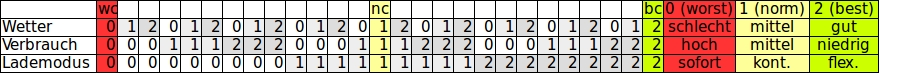
\includegraphics[width=\textwidth]{Szenarien.jpg}
		\caption{Übersicht der variablen Parameter innerhalb der ausgewählten, farblich markierten, Szenarien}
		\label{Abb:Szenarien}
	\end{figure}

\section{Festlegung der Randbedingungen}
	\label{Kap:Festlegung_Szenarien}
	Die szenarienübergreifenden Randbedingungen werden wie folgend definiert und sind abgesehen von der zeitlichen Auflösung tabellarisch in Kapitel \ref{Kap:Konfiguration} gelistet. Die zeitliche Auflösung der Simulation liegt bei 1h, die betrachtete Zeitspanne bei 24~h. Die Netztopologie sowie die Kenndaten der Ladepunkte und der Pufferbatterie entsprechen dem Konzept aus Kapitel \ref{Kap:Vorgaben}. Die Ladepunkte inklusive -regler und Batterie besitzen einen Wirkungsgrad von $\eta_{LP} = 85 \%$. Die maximale Übertragungsrate zwischen Knoten $n1$ mit allen Ladepunkten und der Pufferbatterie und Knoten $n2$ mit PV-Anlage und Netz liegt bei $P_{max,grid} = 50 kW$. Der Algorithmus zur Bestimmung der Nennleistungen für alle Ladepunkte und die Pufferbatterie und für DSM wird aus Kapitel \ref{Kap:DSM} übernommen und um die Wirkungsgrade ergänzt. 
    
    \subsection{Auswahl der Pufferbatterie}
    		Als Pufferbatterie wird aufgrund der in Kapitel \ref{Kap:Akkus} beschriebenen Vorteile ein Bleikristallakku ausgesucht. Es werden drei Akkus des Modells Lead Crystal 6-CNFJ-120 des Herstellers  $\text{Lead Crystal}^{\textsuperscript{\textregistered}} ~\text{Batteries}$ mit jeweils einem IUoU Automatikladegerät (12~V~/~50~A) des Herstellers Fraron für jede Phase ausgewählt. Die Datenblätter sind im Anhang als Abbildung \ref{Abb:datasheet_akku} und \ref{Abb:datasheet_laderegler} gelistet. \\
        
        Die Zellen haben eine Spannung von jeweils 12~V und eine Bruttokapazität von jeweils 100~Ah (1,2~kWh). Die maximal mögliche Ladeleistung je Zelle beträgt 0,6~kW. Die Kosten für Akkuzellen (je 391,90 Euro) und Laderegler (je 299,00 Euro) exklusive Versand liegen zusammen bei ca. 2070,00~Euro. Für die Simulation wird der DoD der Pufferbatterie auf 95~$\%$, der anfängliche SoC der Pufferbatterie auf $50~\%$ und der Lade- und Entladewirkungsgrad inklusive Ladereglerverlusten $\eta_{PB}$ auf $90~\%$ gesetzt.\\
        
        In Tabelle \ref{Tab:PB_Dim} wird anhand der Herstellerangabe der optimale DOD für die 3 oben genannten Akkus mit maximaler Brutto Speicherkapazität über die Lebenszeit berechnet. Zudem wird eine Abschätzung der Rentabilität des Akkus vorgenommen. \\ 
       
        \begin{table}[h]
          \centering
          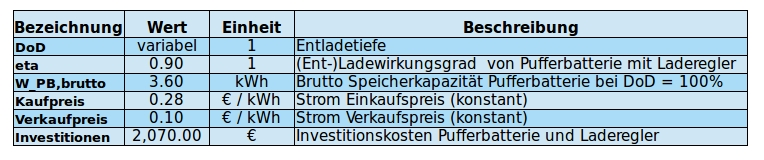
\includegraphics[width=\textwidth]{PB_Dim_stat} \\
          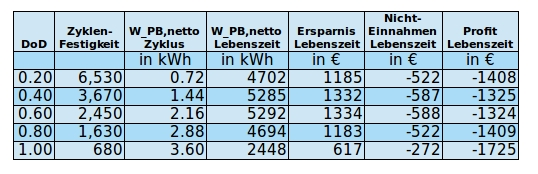
\includegraphics[width=\textwidth]{PB_Dim_dyn}         
          \caption{Bestimmung der optimalen Entladetiefe der Pufferbatterie und Abschätzung des erzielten Profits der Pufferbatterie über die Lebenszeit gerechnet anhand der Zyklenfestigkeit Z}
          \label{Tab:PB_Dim}        
        \end{table}    

		Die Ersparnis ergibt sich aus der Menge nicht eingekaufter Energie und die Nicht-Einnahmen anhand der nicht verkauften Energie über die Lebenszeit. Hierfür wird von einem Kalkulationszins von $0~\%$ und konstanten Strompreisen ausgegangen. Unter den getroffenen Annahmen amortisiert sich die Pufferbatterie nicht innerhalb der Lebenszeit. Bei einem DoD von 60~$\%$ würden sich die Akkus erst bei einem durchschnittlichen Stromkaufpreis von 55,8~$\frac{ct}{kWh}$ - ca. das doppelte heutiger Strompreise - unter sonst gleichen Bedingungen gerade so über die Lebenszeit amortisieren. \\
        
        Um das Betriebsverhalten einer Pufferbatterie in der Simulationsumgebung zu testen werden alle Szenarien trotz nicht wirtschaftlicher Betriebsweise der Pufferbatterie einmal mit den oben spezifizierten Kennwerten berechnet. \\
					
	\subsection{Erzeugungsprofile der PV-Module}
		\label{Kap:Sim_cfg_gen}
		Die Erzeugungsprofile werden anhand der Kenndaten in Tabelle \ref{Tab:PV_kenndaten} der installierten PV-Anlage und den in \ref{Kap:Sim_cfg_gen_data} ausgewählten Globalstrahlungsdaten erstellt, da von der Anlage keine geloggten Erzeugungsdaten über einen längeren Zeitraum zur Verfügung stehen. \\
	
		Der Wirkungsgrad der PV-Module wird modellhaft als konstant angenommen und nach Gleichung \ref{Eq:PV_eta} unter Einsetzen der Kenndaten aus Tabelle \ref{Tab:PV_kenndaten} ermittelt, wobei die Einheiten $W$ und $Wp$ sich herauskürzen. \\
		
			$ \eta_{PV} = (\frac{P_p}{A}) / G_{STC} = (\frac{20145 Wp}{76 \cdot 1,65 m^2}) / (1000 \frac{W}{m^2}) = 16,06 \% $ \\
			
		Die eine Hälfte der Module ist nach Bemessung des Konstruktionsplans in Abbildung \ref{Abb:datasheet_pv_4} unter Annahme einer maßstabsgetreuen Abbildung zu ca. $13,2 \degree$ nach Osten geneigt, während die andere Hälfte symetrisch dazu nach Westen geneigt ist. Zur Einfachheit wird von horizontal angebrachten PV-Modulen ausgegangen. \\
		
		Genauere Ergebnisse können erzielt werden, wenn unter Berücksichtigung der Geoposition, Ausrichtung, Neigungswinkel und Uhrzeit die senkrecht auf die Modulflächen eintreffende Globalstrahlung aus der senkrecht auf die Erdoberfläche eintreffende Globalstrahlung berechnet wird. Die Umrechung der Globalstrahlung von einer ebenen auf eine geneigte Fläche, wie in Kapitel \ref{Kap:G0g} beschrieben, ist noch nicht im Code implementiert. \\			

		\subsubsection{Globalstrahlungsdaten für Mannheim}	
			\label{Kap:Sim_cfg_gen_data}
			Der \ac{DWD} stellt von zahlreichen Wetterstationen Solarstrahlungsdaten (global und diffus), in einer Auflösung von bis zu 10 Minuten auf dem FTP-Server ihres Climate Data Center frei zur Verfügung.\cite{DWD} \\
			
%			Die verwendeten Daten stammen aus Mannheim von der Station mit der ID 05906 und wurden in einer Höhe von 96 m über dem Meeresspiegel am Standort 49.5090° geographischer Breite und 8.5541° geographischer Länge gemessen.\cite{DWD}
			
			Angesichts der Ungenauigkeit der Repräsentativität manuell erstellter Verbrauchs-profile wird eine zeitliche Auflösung von einer Stunde für die dem Erzeugungsprofil zugrunde liegenden Globalstrahlungsdaten als hinreichend genau betrachtet. Eine fest definierte Auflösung von einer Stunde verringert den Programmier- und Rechenaufwand gegenüber höheren oder dynamisch einstellbaren Auflösungen.  \\
						
%			StationsID:	ID 05906 (Mannheim)\\
%			Höhe über dem Meeresspiegel:	96 m\\
%			geographische Breite:	49.5090°\\
%			geographische Länge:		8.5541°\\
					
			Für die Auswahl geeigneter Tage wird mithilfe des in \ref{Kap:Sim_cfg_gen_code} beschriebenen .m-Codes ein Datensatz des DWD mit Tagessummen der Globalstrahlung für die Wetterstation in Mannheim mit der ID 05906 auf 96 m Höhe über dem Meeresspiegel, dem geographischen Breitengrad 49.5090° und geographischen Längengrad 8.5541° untersucht. \\

			Von den verfügbaren Wetterdaten im folgenden Zeitraum wahrer Ortszeit (WOZ) werden die neusten 21 Jahre untersucht: \\
			Zeitraum verfügbar:\quad 	von 01.01.1979 00:00 Uhr \quad bis 01.01.2012 00:00 Uhr \\
			Zeitraum untersucht:\quad 	von 01.01.1991 00:00 Uhr \quad bis 01.01.2012 00:00 Uhr \\

%			Die Datensätze haben laut DWD ein Qualitätsniveau von eins, was bedeutet, dass nur eine formale Prüfung beim Entschlüsseln und Laden der Daten durchgeführt wurde. Im zur Verfügung stehenden Zeitraum sind 78 der 12053 Tage mit inplausiblen Werten versehen.
            
			\subsubsection{.m-Code für Auswertung von Globalstrahlungsdaten}
			\label{Kap:Sim_cfg_gen_code}
            	Das Programm $weatheranalysis.m$ wertet die Globalstrahlungsdaten des DWD mit zeitlicher Auflösung von einer Stunde und einem Tag aus. In einem definierten Zeitintervall der zur Verfügung stehenden Daten sucht der Code den Tag mit der maximalen, minimalen und der geringsten Differenz zur durschnittlichen Globalstrahlung für die Szenarien \ac{WC}, \ac{NC}, \ac{BC} heraus. Zu jedem Tag werden unter Berücksichtigung der Peakleistung der PV-Anlage die Modulerträge ermittelt. Die Ertragsdaten beinhalten keine Wechselrichter- und keine Kabelverluste und werden in einer CSV-Datei mit Zeitstempel gespeichert. \\

Der vollständige Code der Datei $weatheranalysis.m$ wird in Kàpitel \ref{Kap:Code} gezeigt. Das funktionstüchtige Programm mit allen weiteren Dateien für Funktionsdefinitionen und Konfigurationsdaten sind über die beigelegte CD und über Github verfügbar. \cite{github_energyflowsim} Die Benutzer*innen-Anleitung ist einer README Datei beigefügt. \\

%			\lipsum
			\begin{figure}[h]
				\begin{minipage}{0.49\textwidth}
					\centering
					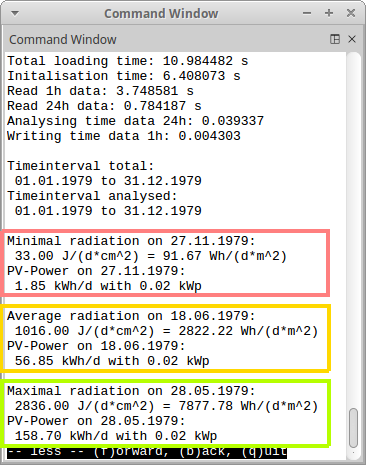
\includegraphics[width=\textwidth]{weather_res_test}
				\end{minipage}\hfill
				\begin{minipage}{0.49\textwidth}
					\centering
					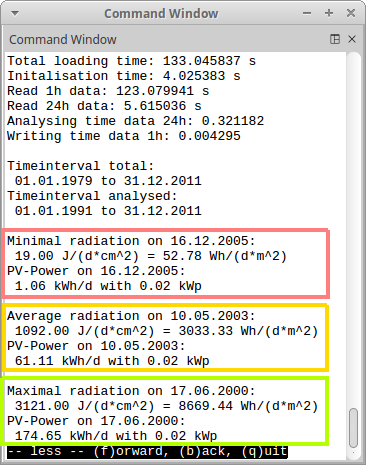
\includegraphics[width=\textwidth]{weather_res}
				\end{minipage}
				\caption{.m-Code Auswertung von Wetterdaten eines Datensatezs über 1 Jahr und über 32 Jahre \\ Farbkennung: Grün: BC, Gelb: NC, Rot: WC}
				\label{Abb:weather_res}
			\end{figure}
%			\lipsum[3]

			Getestet wurde der Code mit einem gekürzten Testdatensatz der einstündigen Wetterdaten im Zeitraum vom 01.01.1979 bis 31.12.1979. Um die Ergebnisse zu überprüfen, wurde der Testdatensatz mithilfe des Tabellenkalkulators Libre Office auf inplausible Datenreihen, minimal, maximal und dem Durchschnitt am nächsten kommende Globalstrahlungsdaten untersucht. Die Auswertung der Testdaten mittels Code in Abbildung \ref{Abb:weather_res} (rechts) und mittels Tabellenauswertung in Abbildung \ref{Abb:weather_verify} sind identisch. Inplausible Daten werden fehlerfrei heraus gefiltert und fließen nicht in die Mittelwertsberechnung oder die Minimasuche ein. \\
						
			\begin{figure}[h]
				\centering
				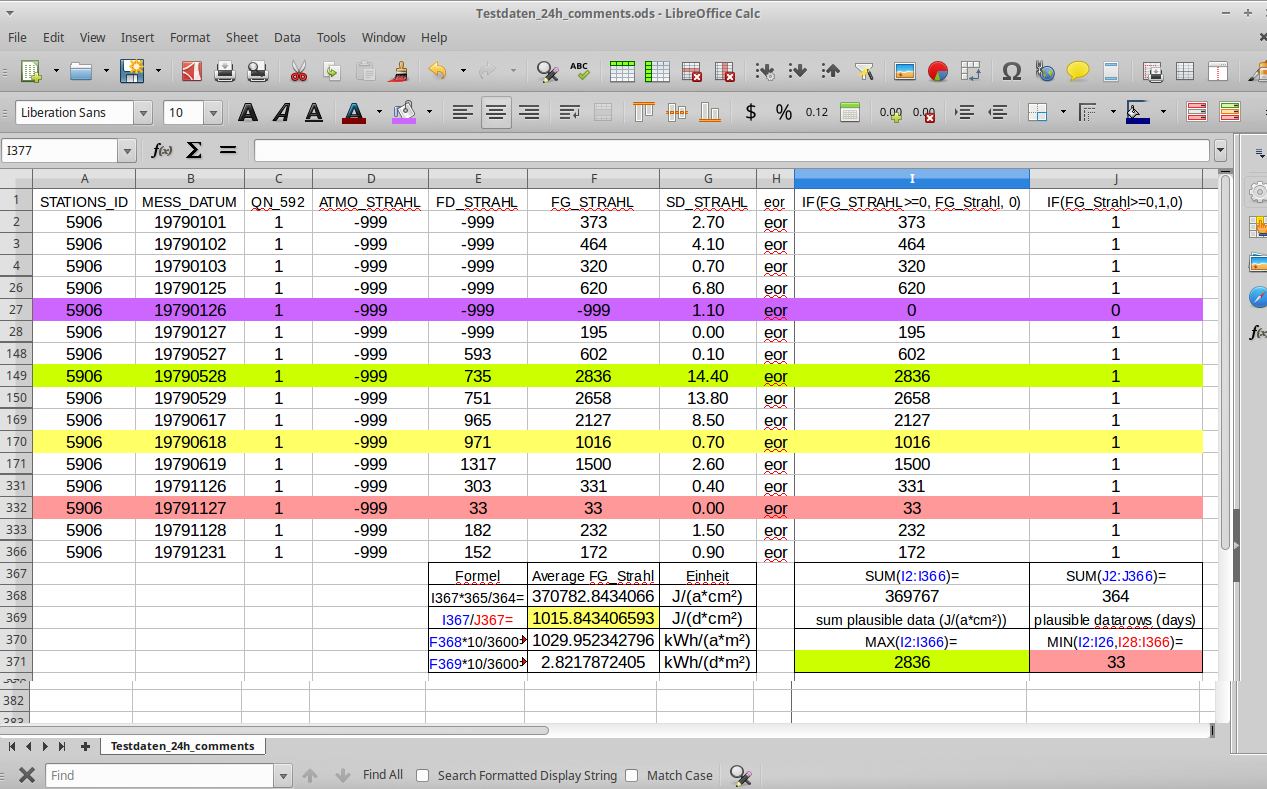
\includegraphics[width=14cm]{weather_verify}
				\caption{
					Überprüfung der Wetterdatenauswertung mit .m-Code in Tabellenkalkulator \\ 
					Farbkennung: Purpur: unplausible Messreihe, Grün: BC, Gelb: NC, Rot: WC \\ 
					ATMO\_STRAHL: Tagessumme der atmosphärischen Gegenstrahlung $\frac{J}{d*cm^2}$\\
					FD\_STRAHL: Tagessumme der diffusen solaren Strahlung $\frac{J}{d*cm^2}$\\
					FG\_STRAHL: Tagessumme der Globalstrahlung $\frac{J}{d*cm^2}$\\
					SD\_STRAHL: Tagessumme der Sonnenscheindauer in $h$\\
				}
				\label{Abb:weather_verify}
			\end{figure}
			
			Die durschnittlich ermittelten Globalstrahlungswerte von ca. 1000 und 1100 $\frac{J}{d*cm^2}$ entsprechen mit etwa $1014\frac{Wh}{a*m^2}$ und $1115\frac{Wh}{a*m^2}$ mit $1\frac{J}{d*cm^2} = \frac{365*100^2}{60^2}\frac{Wh}{a*m^2}$ den typischen Werten für Deutschland zwischen 900 und 1200 $\frac{kWh}{a*m^2}$. \cite{DWD} \\
            
            Die ermittelten Ertragsleistungen $PV-Power$ stellen die Ausgangsleistung der PV-Module dar. Abbildung \ref{Abb:PV_gen} zeigt die Ertragsleistung der PV-Anlage für alle drei Szenarien in Form von Ertragsprofilen mit einem Systemwirkungsgrad von 90\% für Wechselrichter- und Kabelverluste. 

					\begin{figure}[h] % NOTE: Derzeit noch Globalstrahlung in J/cm^2
						\centering
						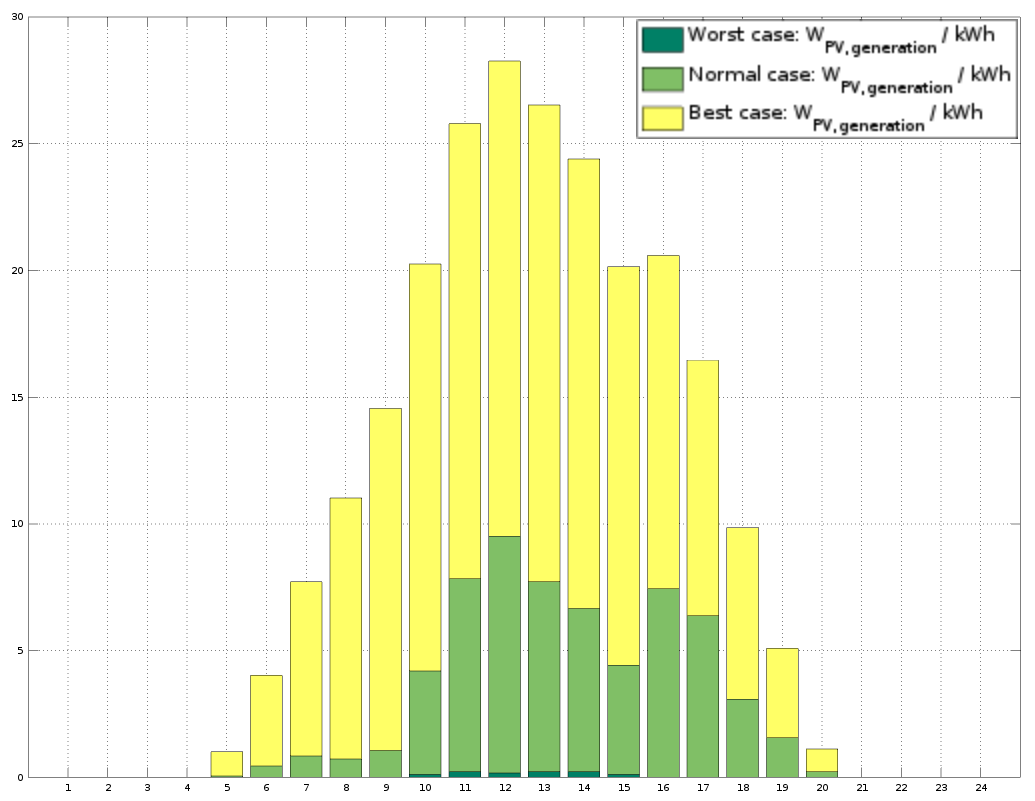
\includegraphics[width=14cm,height=7cm]{W_pv_gen_all}
						\caption{Netto Erzeugungsprofil der PV-Anlage im Worst, Normal und Best Case über 24~h}
						\label{Abb:PV_gen}
					\end{figure}
			
			% NOTE PV Power inplausible!
			
%			Daten: \\
%				Stundensumme der atmosphärischen Gegenstrahlung $\frac{J}{cm²}$\\
%				Stundensumme der diffusen solaren Strahlung $\frac{J}{cm²}$\\
%				Stundensumme der Globalstrahlung $\frac{J}{cm²}$\\
%				Stundensumme der Sonnenscheindauer $min$\\
%				Zenitwinkel der Sonne bei Intervallmitte $Grad$\\
%				Intervallende in WOZ $yyyymmddhh$\\
%				Intervallende in UTC $yyyymmddhh$\\
				

	
	\subsection{Lastprofile der E-Fahrzeuge}
	\label{Kap:Sim_cfg_con}
		Die Lastprofile werden durch das EMS abhängig von den vordefinierten Ladevorgängen, von der eingesetzten Pufferbatterie und von der zur Verfügung stehenden PV-Leistung berechnet. Die Ladevorgänge werden, wie in Kapitel \ref{Kap:DSM} beschrieben, mit den Parametern $t0$, $tT$, $Mode$, $W0$, $Wmax$ und $Pmax$ konfiguriert. Aufgrund der in Realität unterschiedlicher, stark fluktuierender Nutzung werden für die Bestimmung der Szenarien mehrere grobe Annahmen getroffen und ein am Wetter orientiertes Nutzungsverhalten mit Tag- und Nachtladungen modelliert. \\
        
		\begin{figure}[h]
			\centering
			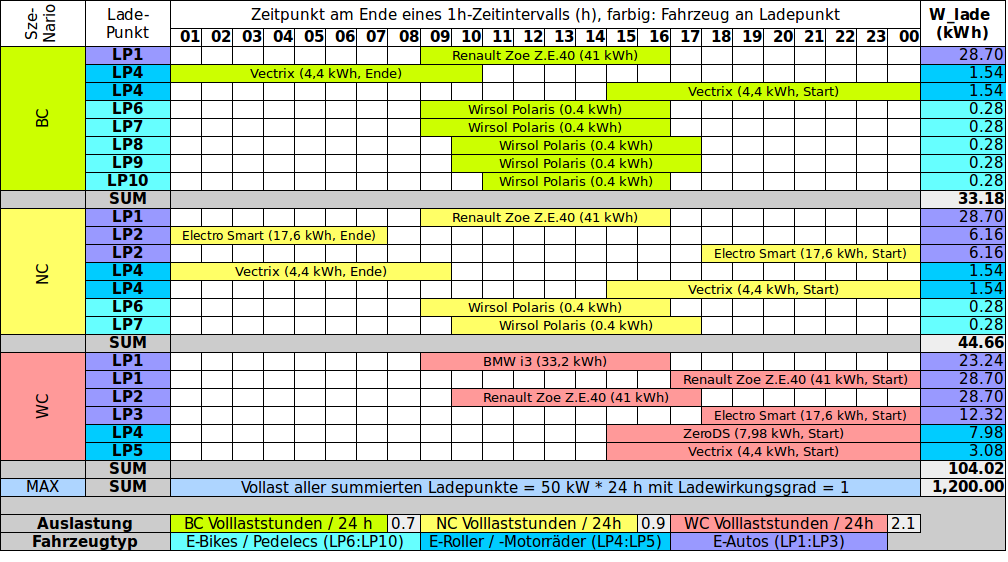
\includegraphics[width=14cm]{Szenarien_last}
			\caption{Ladekonfigurationen für Szenarien BC, NC und WC mit Batteriekapazität $W_{max} = \frac{W_{lade}}{70 \%}$}
			\label{Abb:szenarien_last}
		\end{figure}        
        
        Abbildung \ref{Abb:szenarien_last} zeigt die verwendeten Ladekonfigurationen. Im BC bei gutem Wetter werden 33,18 kWh Batteriekapazität durch ein E-Auto tagsüber, ein E-Roller nachts und fünf E-bikes tagsüber kontinuierlich geladen. Im NC sind es 44,66 kWh bei je einem E-Auto tagsüber und nachts, ein Roller nachts und zwei E-bikes tagsüber, die kontinuierlich geladen werden. Im WC sind es 104,02 kWh bei je zwei E-Autos tagsüber und nachts, sowie jeweils ein E-Roller und ein E-Motorrad abends, die mit maximal möglicher Ladeleistung geladen werden. Der anfängliche SoC aller Fahrzeuge liegt bei $SoC = 30 \% $.\\ 
        				


\section{.m-Code für Simulationen}
	\label{Kap:Code}		
	Das Programm $EnergyFlowSim$ simuliert die Energieflüsse der konzipierten Energieverbundinsel. In Kapitel \ref{Kap:Code} ist dazu ein Programmablaufplan dargestellt. Eine Programmbeschreibung befindet sich im ersten Kommentarblock des Codes der Main File $energyflowsim.m$ in Listing \ref{Code:energyflowsim}. Dazu gibt es beispielhaft den Code $dsmrel.m$ der Funktion $dsmrel()$ in Listing \ref{Code:DSM}.\\

	Alle weiteren Daten für die funktionstüchtige Nutzung des Programms - über 20 Funktionen und 5 Konfigurationsdateien - sind über die beigelegte CD und über Github verfügbar. Die Benutzer*innen-Anleitung ist in einer README Datei. \cite{github_energyflowsim} \\
    
    Sämtliche Funktionen haben in einem auskommentierten Header eine Funktionsbeschreibung und gegebenenfalls Definitionen der Eingangs- und Ausgangsvariablen. Dieser kann in Matlab mithilfe der Funktion $help <Funktionsname>$ abgerufen.\\                

% Easter eggs, also called Paschal eggs, are decorated eggs that are usually used as gifts on the occasion of Easter. As such, Easter eggs are common during the season of Eastertide. Have fun with =).\\

% Eine automatische Dokumentation in Form eines HTML-Wikis mithilfe der Software Doxygen, dem inoffiziellen Standard von Code Dokumentationen, war nicht ohne weiteres möglich. Doxygen ist nicht für .m-Code konzipiert und eine Übersetzung des .m-Codes in doxygen-kompatiblen pseudo C++ Code mithilfe vorhandener Perl Skripte ist trotz mehrfacher Versuche gescheitert.

\section{Simulationen}
	\label{Kap:Simulation}
	\subsection{Energieflüsse der jeweiligen Szenarien}
		Die Simulation berechnet für jede CPS-unit einzeln die stündlichen Energieflüsse. Untersucht werden im weiteren die Energieflüsse an Knoten $n2$ gemäß der Netztopologie in Abbildung \ref{Abb:Netztopologie}. Diese umfassen die Energieflüsse des öffentlichen Versorgungsnetzes (grid), der PV-Anlage (PV) und der Ladeinfrastruktur (node) und sind in Abbildung \ref{Abb:Sim_W_wc} für den Worst Case, in Abbildung \ref{Abb:Sim_W_nc} für den Normal Case und in Abbildung \ref{Abb:Sim_W_bc} für den Best Case dargestellt. Da in allen Szenarien für sämtliche E-Fahrzeuge der selbe Lademodus verwendet wird, gibt es im Fall von Regelbedarf eine Regelstufe in der alle Ladepunkte gleichmäßig abgeregelt werden. \\
		
        \begin{figure}[h]
			\centering
			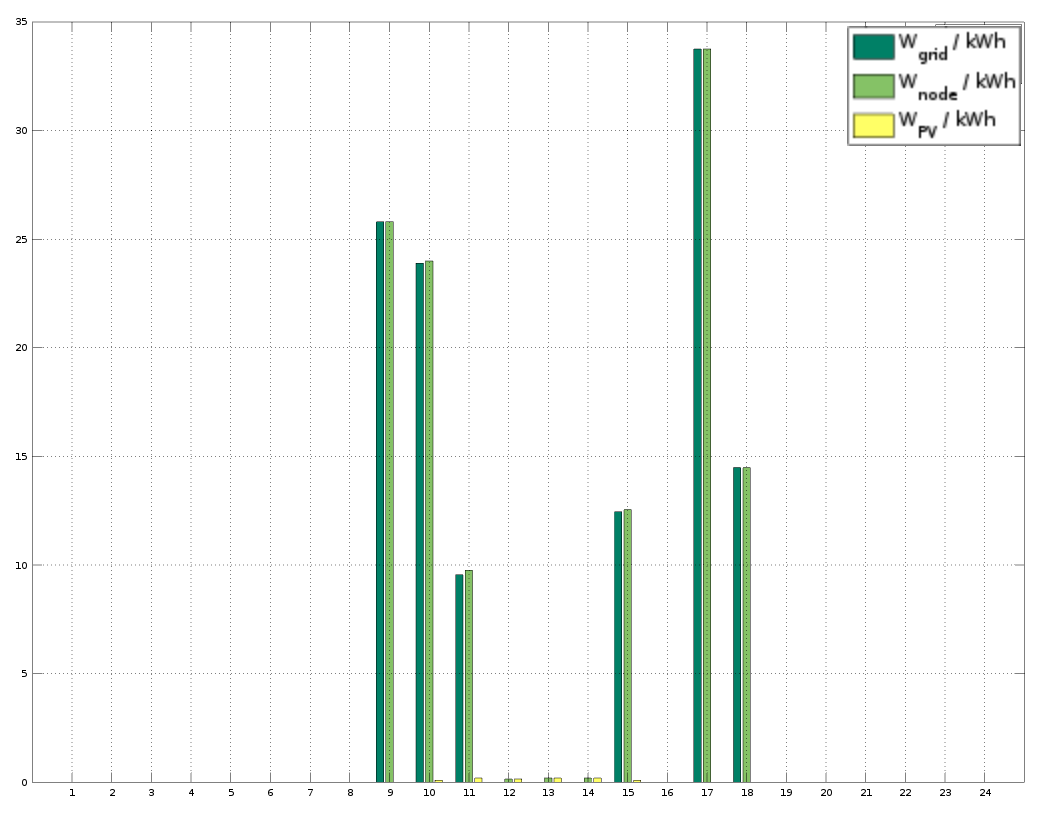
\includegraphics[width=\linewidth,height=8cm]{W_wc}
			\caption{Szenario Worst Case: Stündliche Energieflüsse über 24~h \\ 
            	des öffentlichen Netzes (grid) und der PV-Anlage (PV) im Erzeugerpfeilsystem \\
            	und der Ladeinfrastruktur (node) im Verbraucherpfeilsystem}
			\label{Abb:Sim_W_wc}
		\end{figure}

		\begin{figure}[h]
			\centering
			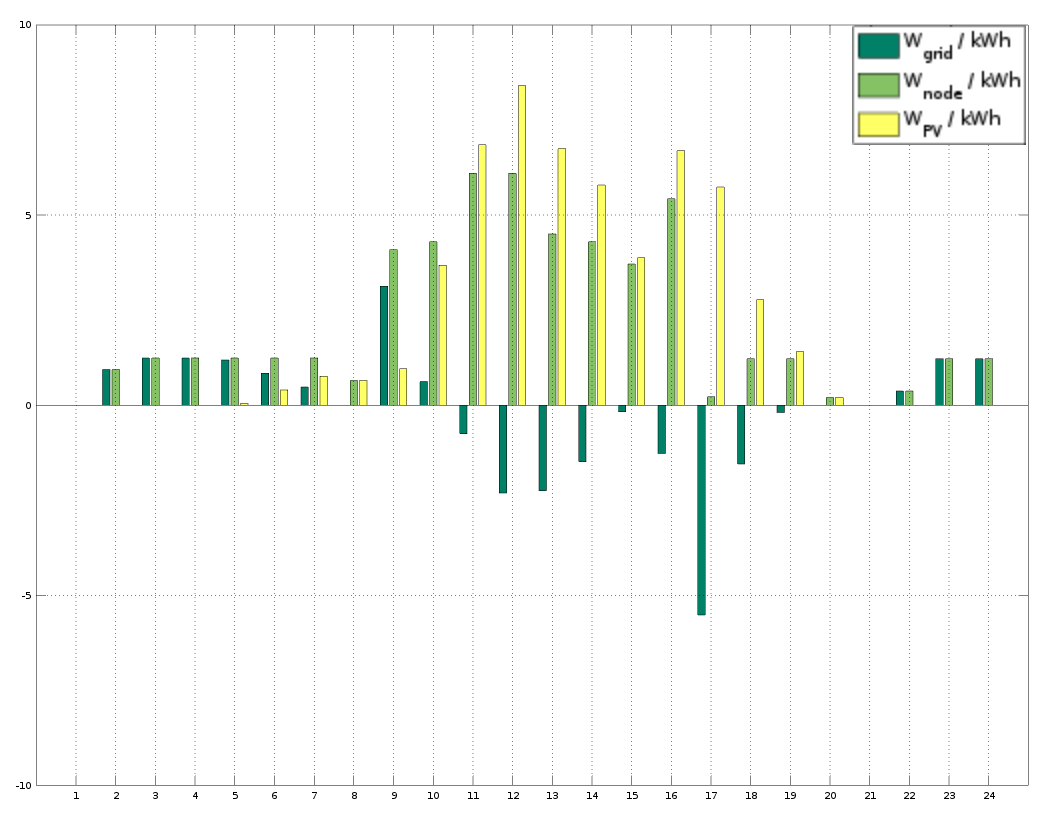
\includegraphics[width=\linewidth,height=8cm]{W_nc}
			\caption{Szenario Normal Case: Stündliche Energieflüsse über 24~h \\ 
            	des öffentlichen Netzes (grid) und der PV-Anlage (PV) im Erzeugerpfeilsystem \\
            	und der Ladeinfrastruktur (node) im Verbraucherpfeilsystem}
			\label{Abb:Sim_W_nc}
		\end{figure}

		\begin{figure}[h]
			\centering
			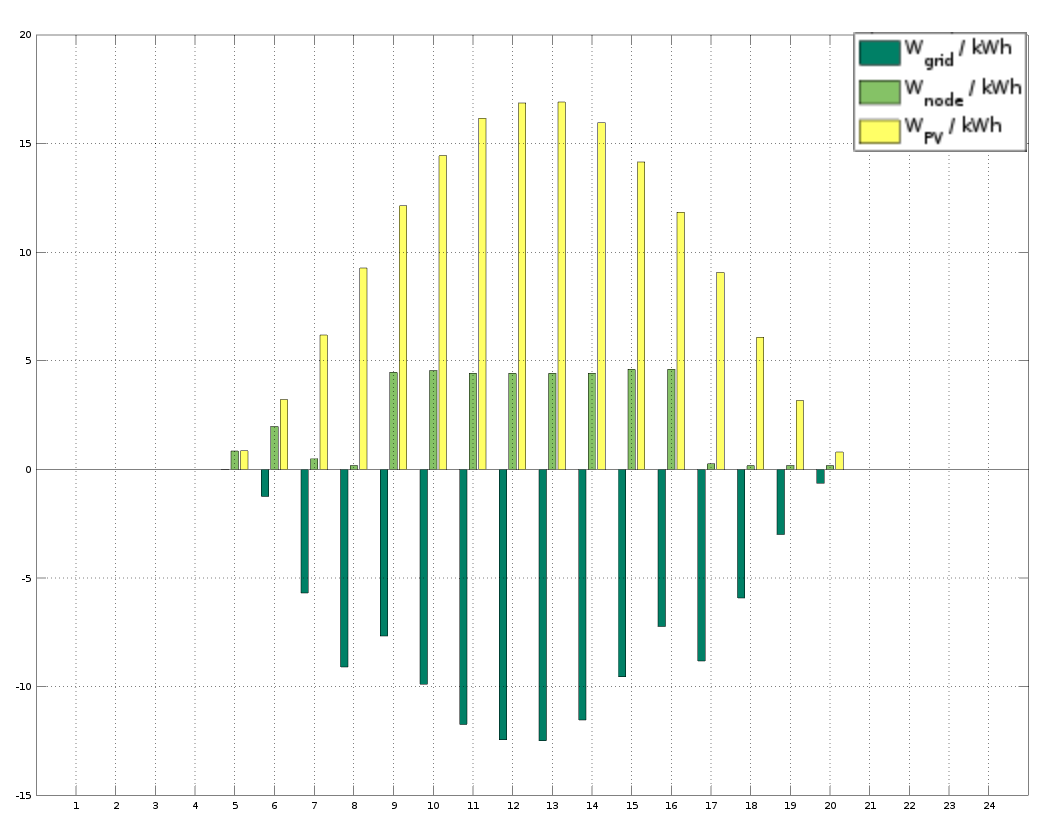
\includegraphics[width=\linewidth,height=8cm]{W_bc}
			\caption{Szenario Best Case: Stündliche Energieflüsse über 24~h \\ 
            	des öffentlichen Netzes (grid) und der PV-Anlage (PV) im Erzeugerpfeilsystem \\
            	und der Ladeinfrastruktur (node) im Verbraucherpfeilsystem}
			\label{Abb:Sim_W_bc}
		\end{figure}

		Für eine bessere Vergleichbarkeit aller drei Szenarien sind die stündlichen Energieflüsse der Ladeinfrastruktur (node) aller drei Szenarien in Abbildungen \ref{Abb:Sim_W_con_all}, der jeweilige Eigenenergieverbrauch der Ladeinfrastruktur in Abbildung \ref{Abb:Sim_W_con_self_all} und jene Energieflüsse des öffentlichen Versorgungsnetzes in Abbildung \ref{Abb:Sim_W_grid_all} dargestellt.\\
        
		\begin{figure}[h]
			\centering
			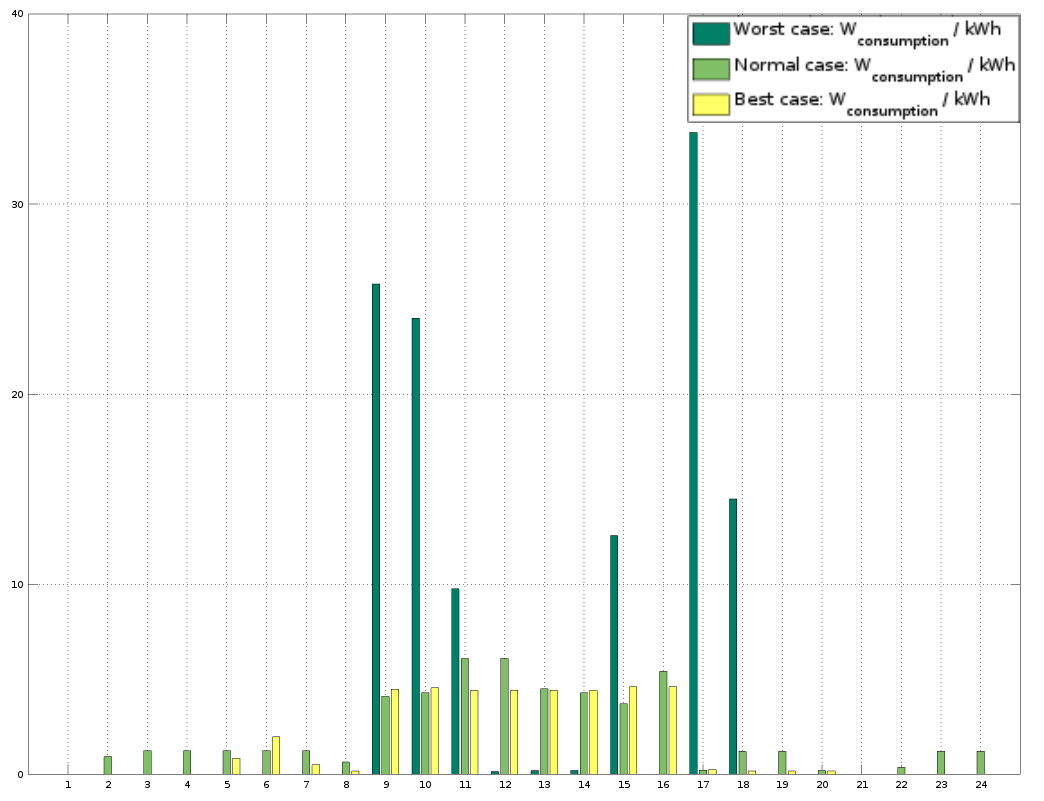
\includegraphics[width=\linewidth,height=8cm]{W_con_all}
			\caption{Stündlicher Energieverbrauch der Ladeinfrastruktur (node) über 24~h \\
            	in den Szenarien Worst Case, Normal Case und Best Case}
			\label{Abb:Sim_W_con_all}
		\end{figure}

		\begin{figure}[h]
			\centering
			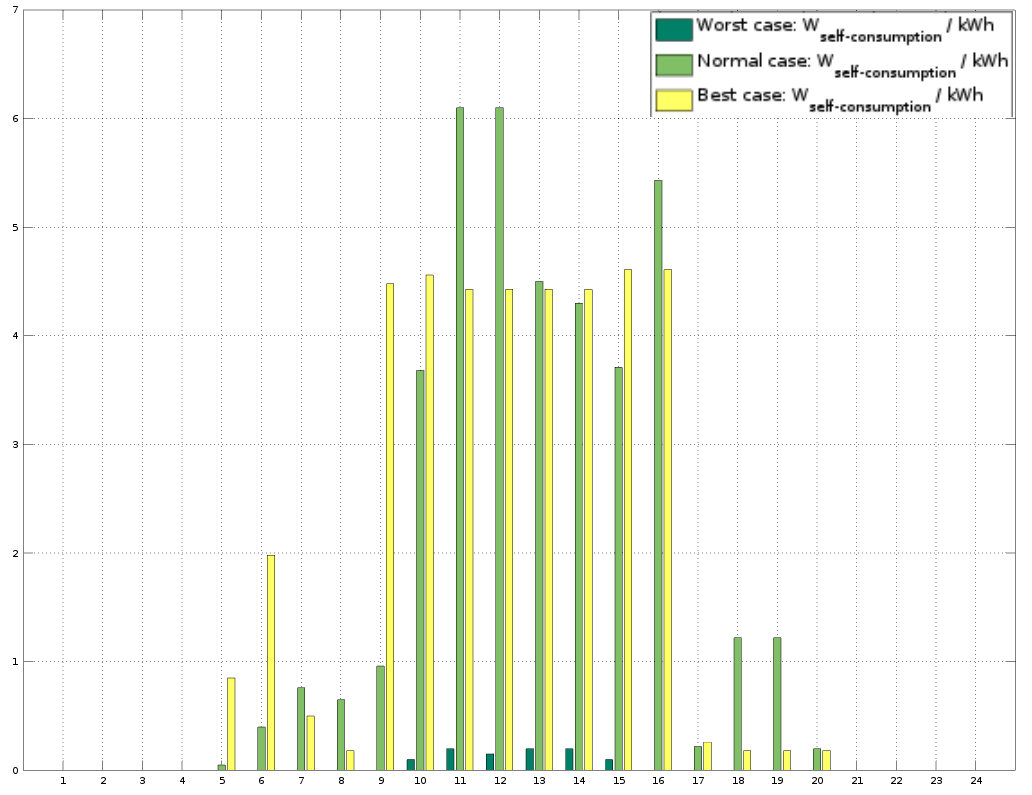
\includegraphics[width=\linewidth,height=8cm]{W_con_self_all}
			\caption{Stündlicher Eigenenergieverbrauch der Ladeinfrastruktur (node) an der PV-Erzeugung (PV) über 24~h \\
            	in den Szenarien Worst Case, Normal Case und Best Case}
			\label{Abb:Sim_W_con_self_all}
		\end{figure}

		\begin{figure}[h]
			\centering
			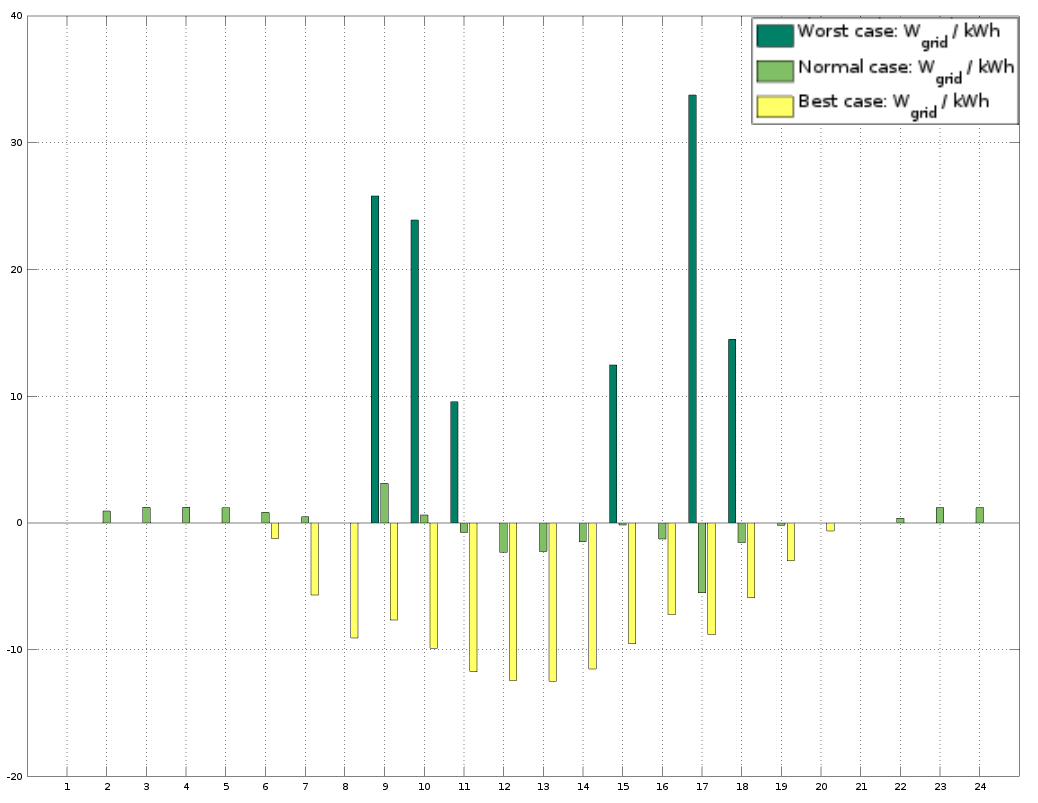
\includegraphics[width=\linewidth,height=8cm]{W_grid_all}
			\caption{Stündlicher Energiebezug vom öffentlichen Netz (grid) über 24~h\\
            	in den Szenarien Worst Case, Normal Case und Best Case}
			\label{Abb:Sim_W_grid_all}
		\end{figure}

	\subsection{Statistiken der einzelnen Szenarien}
		Für eine Gesamtbetrachtung werden die über den Simulationszeitraum summierten absoluten Werte $Gesamtverbrauch$, $Gesamterzeugung$, $Eigenverbrauch$ und die daraus abgeleitete Quotienten $Verh"altnis~~von~~Erzeugung~~zu~~Verbrauch$, $Autarkiegrad$ und $Eigenverbrauchsanteil$ für alle Szenarien ermittelt. \\
        
        Um den Einfluss der Pufferbatterie besser ermitteln zu können, werden zum Einen die Werte $Verbrauch~Pufferbatterie$ und $Erzeugung~Pufferbatterie$ über den Simulationszeitraum $T$ ermittelt. Zum Anderen werden noch drei Szenarien (WC0, NC0 und BC0) ohne Pufferbatterie aber sonst gleichen Bedingungen wie in den Szenarien WC, NC und BC simuliert und deren Statistiken erfasst. \\
        
        Alle Statistiken sind in Tabelle \ref{Tab:Sim_stats} für alle Szenarien gelistet und wurden für alle Szenarien mit Pufferbatterie mit Bereinigung des SoC berechnet. Die Pufferbatterie ist am Ende des Simulationszeitraums unterschiedlich stark geladen. Zur Bereinigung des SoC wird der theoretisch notwendige Eigenverbrauch oder die theoretisch notwendige Erzeugung für Eigenverbrauch zum Wiederherstellen des initialen SoC am Ende des Simulationszeitraums unter Berücksichtigung des (Ent-)Ladewirkungsgrades verwendet. 

        \begin{table}[h]
			\begin{tabularx}{\linewidth}{|X|c|c|c|}
				\hline 
                \multicolumn{4}{|c|}{\textbf{Statistiken Pufferbatterie-SoC bereinigt} } \\
                \hline 
														& \textbf{WC}  & \textbf{NC} & \textbf{BC}  \\ 
				\hline 
				\textbf{Verbrauch Pufferbatterie / kWh}				& 0,55		& 5,21		& 2,79 \\ 
				\hline 
				\textbf{Erzeugung Pufferbatterie / kWh} 			& 1,99		& 5,76		& 1,45 \\ 
				\hline 
				\textbf{Änderung SoC Pufferbatterie / kWh}			& -1,71		& -1,71		& 0,90 \\ 
				\hline 
				\textbf{Verbrauch Pufferbatterie* / kWh}			& 2,45		& 7,11		& 2,79 \\ 
				\hline 
				\textbf{Erzeugung Pufferbatterie* / kWh} 			& 1,99		& 5,76		& 2,26 \\ 
				\hline 
				\textbf{Gesamterzeugung* / kWh} 					& 0,96		& 55,00		& 157.18 \\ 
				\hline 
				\textbf{Gesamtverbrauch* / kWh}						& 122,84	& 53,89		& 39,57 \\ 
				\hline 
				\textbf{Eigenverbrauch* / kWh} 						& 0,96		& 39,51		& 40.38 \\ 
				\hline 
				\textbf{Verhältnis Erzeugung zu Verbrauch* / \%} 	& 0,79		& 105,78	& 389,25 \\ 
				\hline  
				\textbf{Eigenverbrauchsanteil* / \%}				& 100,00	& 71,85		& 25,69 \\ 
				\hline                
				\textbf{Autarkiegrad* / \%} 						& 0,78		& 73,32		& 100,00 \\ 
				\hline 
                \multicolumn{4}{|c|}{\textbf{Statistiken ohne Pufferbatterie} } \\
                \hline 
                										& \textbf{WC**}  & \textbf{NC**} & \textbf{BC**}  \\ 
				\hline 
				\textbf{Gesamtverbrauch / kWh}						& 122,38	& 52,54		& 39,04 \\ 
				\hline 
				\textbf{Eigenverbrauch / kWh} 						& 0,40		& 34,47		& 37,59 \\ 
				\hline 
				\textbf{Verhältnis Erzeugung zu Verbrauch / \%} 	& 0,78		& 104,67	& 402,66 \\ 
				\hline  
				\textbf{Eigenverbrauchsanteil / \%}					& 42,11		& 62,69		& 23,91 \\ 
				\hline                
				\textbf{Autarkiegrad / \%} 							& 0,33		& 65,61		& 96,29 \\ 
				\hline                
			\end{tabularx} 
			\caption{Statistiken der simulierten Szenarien Worst (WC), Normal (NC) und Best (BC) Case \\
            		*SoC der Pufferbatterie bereinigt mit SoC(Startzeit) = SoC(Endzeit) \\
                    **Szenarienbedingungen gleich WC, NC und BC ohne Verwendung einer Pufferbatterie}
			\label{Tab:Sim_stats} 
		\end{table}	



